%%%%%%%%%%%%%%%%%%%%%%%%%%%%%%%%%%%%%%%%%%%%%%%%%
%%%%%%%%%%%% cap: application %%%%%%%%%%%%%%%%%
%%%%%%%%%%%%%%%%%%%%%%%%%%%%%%%%%%%%%%%%%%%%%%%%%

\chapter{Creating a BCI Application Platform}\label{cap:development}
In this bachelor's thesis, the main objective is creating a BCI App Platform, meaning the creation of a program that is able to open other applications while interfacing with the Unicorn Hybrid Black, a Brain Computer Interface, to receive input from a disabled user via a P300 speller. The user can navigate through his favourite applications which are displayed on the platform's graphical user interface using the Unicorn Speller, g.tec's own implementation of the P300 speller. Using the speller, he can then select an application to launch and use for as long as he desires, after which he can once again close it through the speller's board by looking at its elements. The results show a stable application that can be used to navigate through compatible apps and open them with ease.

\section{Platform Architecture}
The application to be implemented makes use of a BCI Speller, namely the Unicorn Speller that is part of the Unicorn Suite Hybrid Black. This speller can only be used with the Unicorn Hybrid Black Brain Computer Interface. The speller is used as the primary and only input method for a disabled user to interact with the application. The BCI headset sends its output (the item the user selected from the board) through a UDP server to a specific IP address and port combo specified in the speller settings. The application implements a UDP listener that runs as a background process of the application, waiting for an input from the user. When aforementioned input arrives, the listener sends it to the application which then interprets it accordingly.
\vspace{\baselineskip}\newline
The platform itself is a Unity application that when run fetches all BCI applications installed on the user's disk and displays them to the user so that he/she can select one. Once an application is selected, the platform simply runs it and locks all user input, as the applications housed inside also interface with the speller and by keeping input unlocked, the user may accidentaly open multiple apps or cause other unwanted behaviour.

\begin{figure}[H]
  \centering
  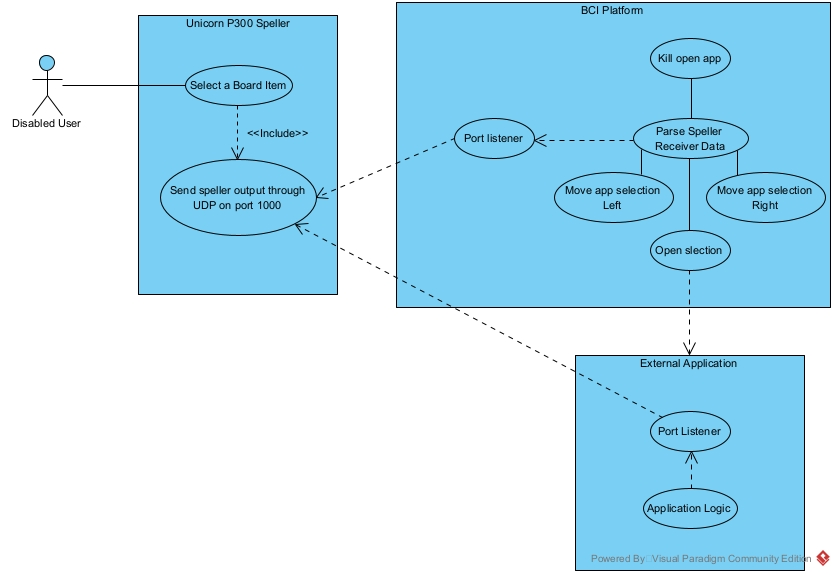
\includegraphics[width=1\textwidth]{Diagrams/Platform Use Case.jpg}
  \caption{Platform use case diagram}
\end{figure}
\begin{figure}[H]
  \centering
  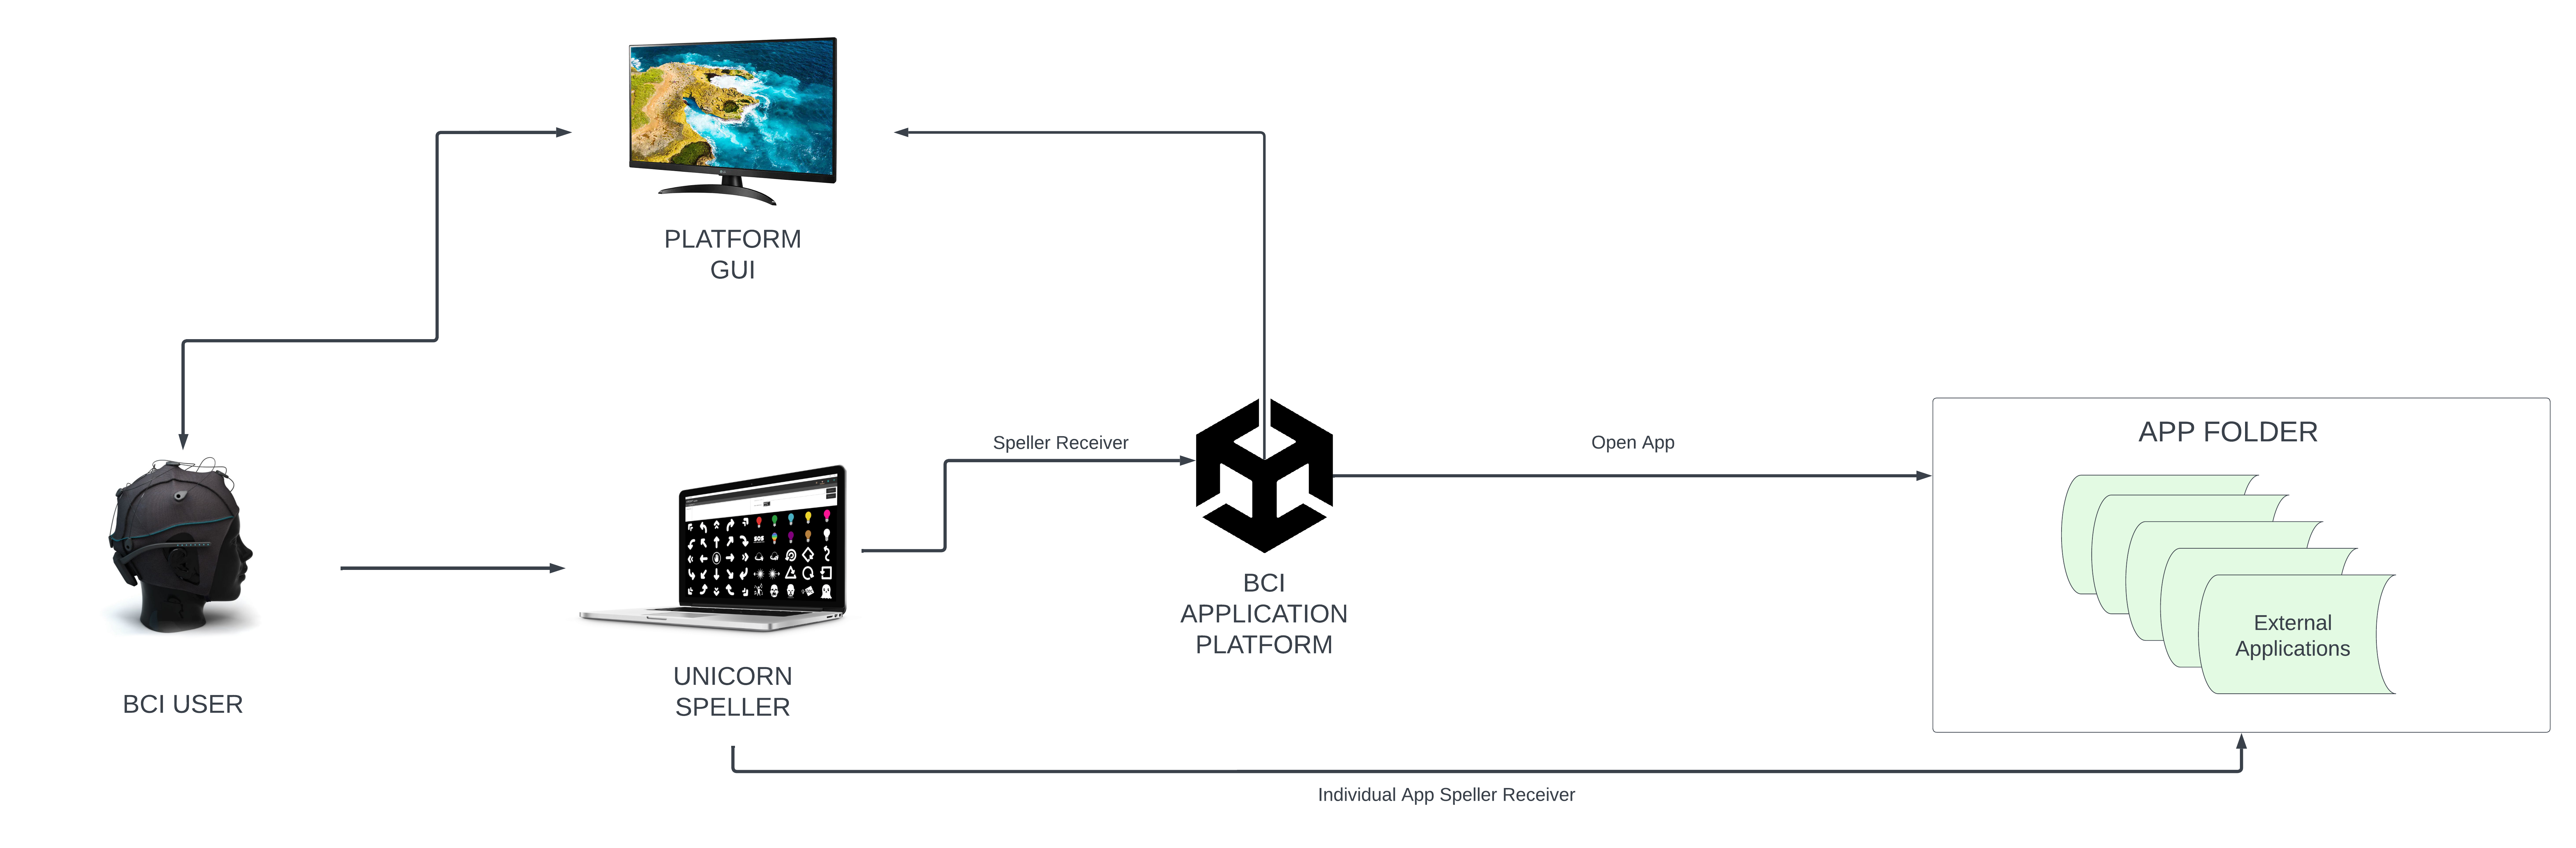
\includegraphics[width=1\textwidth]{Diagrams/Platform Architectural Diagram.png}
  \caption{Architectural Diagram}
\end{figure}


\section{Implementation Details}
The Platform is built and run using the Unity Engine and all scripting is done in the C\# programming language. The engine ensures great control over the UI elements on the front-end of the application and stability in the back-end.

\subsection{Game Objects and UI}
In order to display all the applications to the user, they need to be in a centralised location, where the platform can locate them and show them to the user. The location picked for this purpose is inside the User's Documents directory, in a directory called \textit{.bciapps}. Inside here, all applications sit in their separate folder. Furthermore, in order to automate the platform better, a similar file structure was used between each of the applications, where every application folder contains an \textit{app.exe} file, which is the app executable file called by the platform when the user decides to open that specific app, and another \textit{icon.png} which is that specific application's icon that is being displayed inside the platform to the user. This file structure is reminiscent of other software platforms, such as steam, which use specific directories to store their applications.
\subsubsection{The App Class}
An App.cs file was created in order to store all information about a specific application present in the .bciapps folder. This class contains member variables for the application name as well as member variables for both the absolute path of the app's executable file and its icon file. The class also contains a member function called run(), which is used in order to start the application when the user selects it and decides to do so via Unity's Process.Start() function.
\subsubsection{App Prefabs and Management}
An empty game object was created to house Manager.cs, a C\# script used to manage all apps. Another game object, a prefab, is created with a Sprite Renderer. This prefab will serve as the base for all app Game Objects when they get instantiated. 
\vspace{\baselineskip}\newline
Before the main game loop starts, in the Start() function provided by Unity, this script browses the .bciapps directory and for each application it creates a new App type object which it then stores in a list. The list of apps get instantiated inside of a container Game Object, with each icon file getting transformed into a Texture2D type, which is then fed to the Sprite Renderer to display the icon to the user[see listing 3.1].

\begin{lstlisting}[language={[Sharp]C}, caption={Manager.cs initialisation}, label={Script}]
    void Start() {
        userPath = getUserPath();
        string[] folders = Directory.GetDirectories(userPath);

        string app;
        string icon;
        foreach (string folder in folders) {
            app = folder + "\\app.exe";
            icon = folder + "\\icon.png";
            App newApp = new App(folder, app, icon);
            newApp.debugPrint();
            apps.Add(newApp);
            appCounter++;
        }
        int xpos = 0;
        foreach (App i in apps) {
            var newObj = GameObject.Instantiate(prefab, new Vector3(xpos, 0, 0), Quaternion.identity);
            byte[] fileData;
            if (File.Exists(i.iconPath)) {
                fileData = File.ReadAllBytes(i.iconPath);
                Texture2D texture = new Texture2D(1, 1);
                texture.LoadImage(fileData);
                Sprite sprite = Sprite.Create(texture, new Rect(0, 0, texture.width, texture.height), new Vector2(0.5f, 0.5f));
                newObj.GetComponent<SpriteRenderer>().sprite = sprite;
            }
            newObj.transform.parent = container.transform;
            xpos += 3;
        }
    }
\end{lstlisting}

In order to make the UI reflect the change in the user choice, the whole container Game Object in which the application instances are housed is moved with the user's input. This simple approach[see listing 3.2] using a container app makes it easier to instantiate all applications without having to worry about moving each one every time the user changes his/her selection.

\begin{lstlisting}[language={[Sharp]C}, caption={Manager.cs initialisation}, label={Script}]
    public void moveContainer(Direction direction)
    {
        if(direction == Direction.RIGHT) {
            container.transform.position = new Vector3(container.transform.position.x - 3, 0, 0);
        }
        if(direction == Direction.LEFT) {
            container.transform.position = new Vector3(container.transform.position.x + 3, 0, 0);
        }
    }
\end{lstlisting}


\subsection{Speller Receiver}
The Unicorn Speller outputs via network using UDP. In order to get the user's input signals, we must implement a UDP port listener that always listens on port 1000 (the default port of output on the speller). The Receiver.cs script and the implementation of the port listener must run asynchronously, alongside the main platform program, as a synchronous run can brick the whole Unity editor and/or final built application until an input is received. Since this is not a behaviour that is compatible with the solution presented, a separate process is created to run the receiver script.
\begin{lstlisting}[language={[Sharp]C}, caption={Manager.cs initialisation}, label={Script}]
    // big implementation goes here
\end{lstlisting}


\subsection{Speller Board}
In order to use the platform, we must first load the custom board \textit{platform.ibc} into the speller. To do so, we simply select the cog menu in the top left of the speller, selecting "Board and timing...". Inside this new window, we click the "Load" button in the bottom left of the window and we select the aforementioned .ibc file. As this is part of the initial app setup, this obviously cannot be done by a disabled individual without help. The upside of the Unicorn speller is that once a board is set, the speller always loads the last configuration, so this step is a "set it and forget it" part of the setup.
\vspace{\baselineskip}\newline
The Platform speller consists of a full QWERTY style keyboard and a navigation pad on the right hand side of the keyboard. This may seem a bit excessive for a simple platform and that is because it is. The applications inside of the platform use the speller for input as well, all of them implementing their own receivers. This would be a non-issue if the board file could be changed during run-time, but it cannot as the speller settings cannot be changed while the speller itself is running. Scripts could be created to automate this, but scripts can fail and in the event of such failure, an able-bodied person would have to step in, which is unsatisfactory. This creates an issue in the implementation where either all apps have to be designed to work with the same style of board (which would mean app integration takes longer, as each individual app's receiver code needs to be changed) or a umbrella board that covers all bases needs to be created. In this implementation I have opted to create such a board that covers all needs.



\section{Example run}
\subsection{Initial Setup}
Before a disabled user can use the application on their own, an initial setup must be preformed with the help of an able-bodied individual.
